\documentclass{article}
\usepackage{jim}
\usepackage{microtype}
\usepackage{fontspec}
\usepackage{graphicx}
\usepackage{hyperref}
\usepackage[french]{babel}
\fontspec{Times New Roman}
\usepackage[greyscale]{xcolor}

\usepackage{pdflscape} %\landscape latex
\usepackage{caption}
\usepackage[a4paper]{geometry}
\usepackage{subcaption}
\usepackage{listings}
\selectcolormodel{gray}


\title{Présentation du projet \textsc{Inalaya}}
\author{\emph{Jean-Michaël Celerier} \\  Blue Yeti, F-17110 France. \\ jeanmichael@blueyeti.fr }
\date{}
\begin{document}
    \maketitle
    \section*{Présentation}
    \textsc{Inalaya} vise à proposer une expérience sensible par l’ajout d’une couche sonore interactive sur 
    un objet de référence : image, objet matériel, contenu visuel numérique, ou environnement.
    Cette couche audio interactive est gérée par un scénario complexe : prise en compte 
    des  actions des utilisateurs, contraintes temporelles, contraintes spatiales, conditions, 
    embranchements, boucles, multi-entrées. 
    Ce scénario peut être créé par une ou plusieurs personnes en prenant en compte les caractéristiques de l’objet de référence.
    
    Concernant l’écriture et l’exécution de scénarios complexes, des travaux de recherche ont eu lieu 
    dans le cadre du projet \textsc{OSSIA} (Open Scenario System for Interactive Applications) soutenu 
    par l’agence nationale de la recherche.
    L’un des objectifs de ce projet a été d’offrir aux développeurs des outils génériques pour l’écriture de scénarios d’interactions complexes et l’exécution de ceux-ci, notamment via le développement du logiciel \textsc{i-score}\footnote{www.i-score.org}.
    
    En amont du projet OSSIA, Blue Yeti a effectué un premier travail sur la création de scénarios 
    audio basés sur des paramètres d’espace, utilisant la géolocalisation de l’utilisateur pour 
    naviguer dans un scénario s’exécutant sur terminaux mobiles iOS.
    
    Ce document présente un démonstrateur qui ajoute une couche sonore interactive au tableau \emph{Le Jardin des Délices} de Jérôme Bosch.
    Nous détaillerons l'approche, les contraintes techniques, et les différents cas sonores qui peuvent être rencontrés en parcourant l'\oe uvre.

    \subsection*{Blue Yeti}
    Blue Yeti conçoit et développe des dispositifs interactifs multimédia, visuels et sonores, dédiés à des usages culturels, éducatifs et artistiques.
    Blue Yeti intervient auprès des scénographes, enseignants, musées, centres scientifiques, collectivités, laboratoires de recherche, artistes et centres de création pour la conception et le développement d'installations multimédia et d’espaces immersifs interactifs, basés sur des technologies telles que interfaces tactiles multitouch, interaction sans contact, réalité augmentée, périphériques mobiles.
    Créée en 2007, l'entreprise est actuellement constituée d’une équipe de 6 personnes permanentes et d’un réseau de développeurs indépendants, designers sonores et artistes visuels qui apportent leur créativité et leur savoir-faire technique en fonction des spécificités de chaque projet.
    
    Blue Yeti possède également des compétences dans le domaine de la captation et l’analyse temps 
    réel du geste, ainsi que dans le mapping entre geste et processus sonores. Ces compétences ont 
    été acquises durant la thèse de Jean-Michel Couturier, co-gérant de Blue Yeti (thèse effectuée au 
    laboratoire de Mécanique et d’Acoustique de Marseille, soutenue en 2004) et consolidées par la suite dans différents projets de l’entreprise.
    \section*{Démonstrateur}
    \begin{figure*}[h]
        \centering
        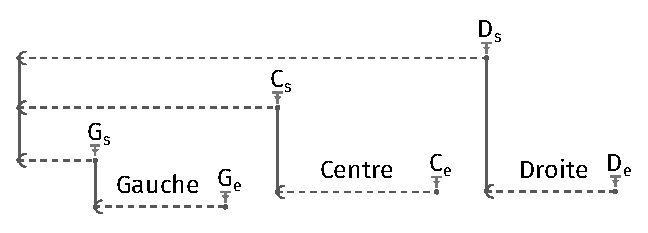
\includegraphics{images/1stcase.eps}
        \caption{Structure de haut niveau dans i-score. Cette structure est contenue dans une contrainte infinie pour que l'installation ne prenne jamais fin. Les trigger point $G_s$, $C_s$, $D_s$ sont les conditions d'entrée du panneau. Par exemple, pour le panneau central, la condition est \lstinline{/mouse/x > 480 et /mouse/x < 1440}. De même, $G_e$, $C_e$, $D_e$ sont les conditions de sortie. La condition est la négation de la condition d'entrée : \lstinline{/mouse/x <= 480 ou /mouse/x >= 1440}.}
        \label{fig.1stlevel}
    \end{figure*}
    Jérôme Bosch est un peintre néerlandais du début de la Renaissance.
    Nous avons choisi pour ce démonstrateur de mettre en application les travaux menés dans le projet Inalaya, sur le fameux triptyque \emph{Le Jardin des Délices}, dont la création est généralement datée entre 1500 et 1515. 
    Faisant preuve d'une richesse en terme de détails et de situations distinctes peu courante, dans un style rappelant parfois des œuvres surréalistes beaucoup plus récentes, ce tableau nous a semblé idéal pour expérimenter les outils développés et les approches choisies.
    
    Pour ce faire, nous proposons aux spectateurs d'interagir avec une surface tactile et de découvrir les différentes couches sonores qui ont été apportées au tableau soit via un casque, soit via une paire d'enceintes.
    Certaines couches sont statiques et d'autres sont dynamiques : des petits scénarios sont présents dans le tableau, et différentes successions d'évènements et d'interactions peuvent conduire à des résultats sonores différents.
    
    \subsection*{Enjeux}
    Les enjeux pour ce projet sont de découvrir les limites et problèmes techniques qui se posent lors de l'utilisation d'un outil principalement temporel (i-score) pour décrire des scènes spatiales.
    L'interface d'i-score est en soi relativement complexe : dans une seule time-line, se superposent des graphes logiques, temporels, et de données, qui sont liés par un faible nombre d'éléments de syntaxe.
    À cela, nous rajoutons une couche de données spatiales.
    
    Un second objectif est d'étudier le comportement d'i-score dans un cadre majoritairement interactif.
    C'est-à-dire que nous cherchons à écrire une partition qui décrit non pas un morceau de musique avec une durée finie et un séquençage plus ou moins ordonné, mais un programme interactif qui est quasiment tout le temps en boucle ouverte : à chaque instant, le spectateur peut interagir avec l'installation. 
    
    %\begin{itemize}
    %\item bosch
    %\item décliner éléments qui sont interactifs
    %\item quelle interaction 
    %\end{itemize}
    \section*{Méthode}
    Nous utilisons un ensemble d'outils fonctionnant en concert pour réaliser cette installation.
    Le chef d'orchestre est i-score.
    Cependant, ce n'est pas suffisant.
    Les fonctionnalités suivantes sont gérées par une flotte de programmes externes : 
    \begin{itemize}
        \item Gérer l'interaction en entrée.
        \item Produire du son (spatialisé ou non).
        \item Gérer des scènes d'objets en trois dimensions avec des sources sonores.
    \end{itemize}
    
    Ces programmes communiquent avec i-score via les protocoles OSC et Minuit.
    Nous avons notamment utilisé Qt pour l'entrée utilisateur et la création de scènes 3D avec des sources sonores spatialisées, via \textbf{Qt3D} et \textbf{QtAudioEngine}.
    \textbf{OpenFrameworks} et notamment l'extension \textbf{ofxMaxim} qui permet d'utiliser la bibliothèque Maximilian~\cite{grierson2010maximilian} pour différents effets de synthèse.
    
    Une des limitations actuelles est la difficulté de router dans un autre logiciel la sortie audio d'un moteur de spatialisation 3D orienté objet tel que \textbf{Unity3D}, \textbf{Unreal Engine}, ou \textbf{Qt3D} : ces outils sont prévus pour produire des applications qui sortent directement sur une carte son.
    
    \subsection*{Écriture et création}
    \begin{figure}[h]
        \centering
        
        \includegraphics[height=8cm]{images/2ndcase.eps}
        \caption{Version simplifiée de la contrainte qui gère la partie supérieure-gauche du tableau. On trouve en haut un processus Scénario et en bas un processus Espace.}
        \label{fig.2ndcase}
    \end{figure}
    L'écriture pour ce tableau sonore interactif repose sur la notion de calques.
    Il y a trois premières zones distinctes, qui sont les trois panneaux du tryptique.
    
    Puis, dans ces zones, on sépare le tableau en plans; cette séparation est décrite dans les figures en annexe de ce document.
    
    Chaque panneau va posséder une première ambiance sonore discrète, puis chaque plan va lui-même 
    posséder une ambiance de fond plus marquée qui s'y superpose.
    Enfin, différents objets interactifs seront placés au premier plan en terme de mixage.
    
    
    Le premier niveau d'écriture peut se faire uniquement à l'aide de la syntaxe propre à i-score : 
    sachant que l'on dispose des coordonnées du pointeur sur le tableau, on peut écrire la structure visible en fig.~\ref{fig.1stlevel}.
    Chacune des contraintes temporelles, en bleu pointillé, contient par la suite les données propres à ce panneau, et des états de début et de fin produisent des sons de transition.
    
    Enfin, une fois entré dans un panneau, un scénario déclenche un fondu d'une seconde sur le son d'ambiance correspondant.
    
    \begin{figure}
        \centering
        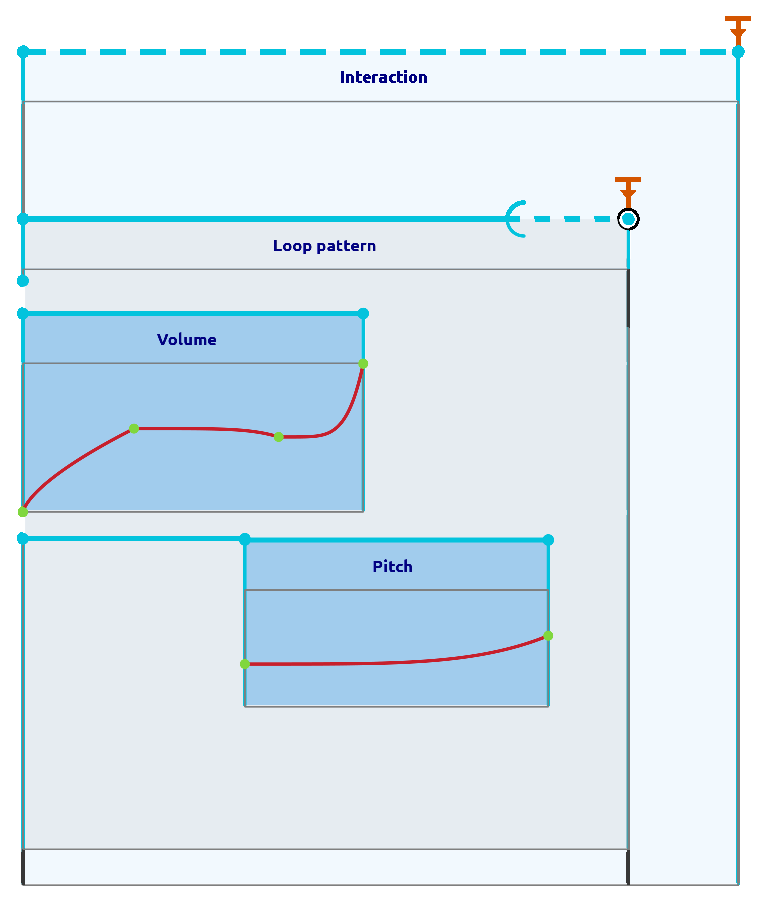
\includegraphics[height=6cm]{images/trigger.eps}
        \caption{Patron pour déclenchement et traduction d'évènements. Une boucle dont la contrainte parente est souple contient un trigger de fin ayant pour condition de déclenchement le message source, et déclenche un état qui va générer le message cible. Une fois cet état envoyé, un bref scénario s'exécute, puis l'attente pour un nouveau message recommence.}
        \label{fig.trigger}
    \end{figure}
    
    On décrit par la suite à titre d'exemple le scénario utilisé pour la zone haut-gauche.
    Dans ce scénario, en fig.~\ref{fig.2ndcase}, on trouve plusieurs zones interactives ellipsoïdes : ce sont des animaux qui produiront un son lors d'une collision du pointeur.
    
    La logique est représentée de manière séparée, dans le scénario situé au dessus de la zone d'espace.
    Notamment, pour les collisions, on dispose d'une boucle qui contient un trigger : c'est le patron de conception qui sert à traduire un évènement interactif en un autre évènement dans i-score. Nous associons de plus parfois des automations permettant de contrôler volume et hauteur des échantillons correspondant aux sons d'animaux. 
    Un exemple est donné en fig.~\ref{fig.trigger}.
    
    Enfin, la distance du curseur à la zone rectangulaire permet de modifier un paramètre de synthèse du son qui semble émaner du pilier central, tandis que la collision a pour effet de déclencher les sons de tous les animaux via une interaction séparée.
    
    \section*{Conclusion}
    Le développement de ce projet a fait apparaître des impératifs pour la réalisation efficace de sonifications d'\oe uvres d'art. 
    Notamment, la disjonction entre la logique et le visuel du tableau force l'auteur à annoter énormément la partie logique pour ne pas commettre d'erreurs.
    
    Cependant, la méthode proposée permet de développer des sonifications rapidement; une prochaine étape est l'intégration des outils de création sonore directement dans i-score pour ne pas avoir à gérer une flotille de programmes et qui ne dépendrait pas de protocoles de communication réseau. En effet, cela rajoute une certaine complexité : gestion des ports réseau, etc.
    
    Enfin, une approche alternative serait de se baser principalement sur un outil d'écriture à dominante spatiale, comme par exemple le moteur de jeu Unity3D, et de décliner plusieurs petits scénarios i-score qui gèreraient chacun une partie de la scène. 
    Cette inversion de rôles peut avoir des avantages, comme une vision globale de la scène, et aussi des inconvénients : il devient plus dur d'organiser des interactions entre objets distincts s'ils sont gérés par des scénarios séparés.
    
    \section*{Références}
    \bibliographystyle{plain}
    \bibliography{inalaya}
    \newpage{}
    {
    \begin{figure}
        \centering
        \begin{subfigure}[t]{0.45\textwidth}
\centering
\begin{subfigure}[t]{\textwidth}
    \centering
    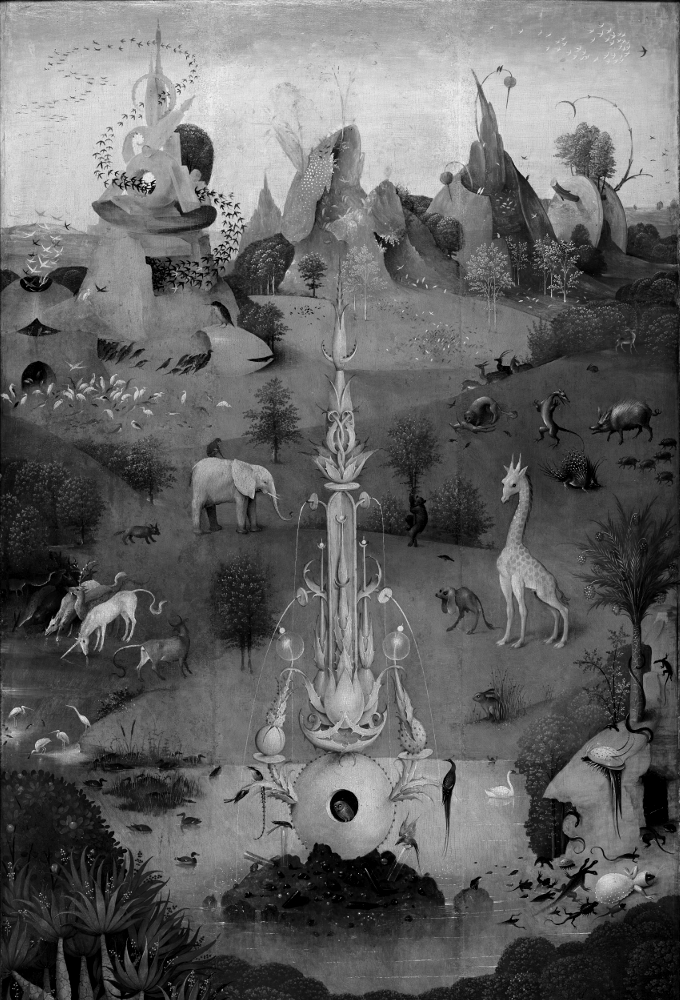
\includegraphics[width=\textwidth]{images/A1.png}
    \caption{Une première perspective marquée et s'étendant au loin. Ici, l'auditeur peut explorer une ménagerie positionnée en trois dimensions, ainsi que des sons doux émanant de la structure centrale.}
    \label{fig.a1}
\end{subfigure}~\\       
\begin{subfigure}[t]{\textwidth}
    \centering
    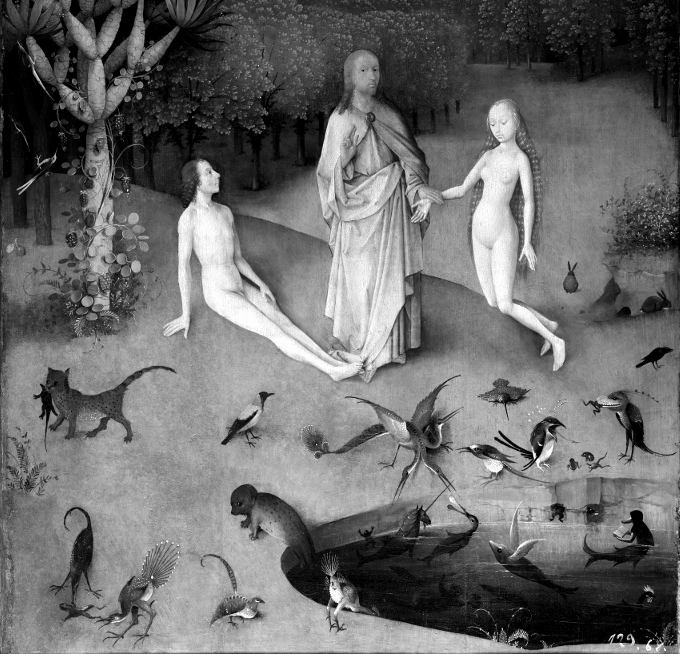
\includegraphics[width=\textwidth]{images/A2.png}
    \caption{Une scène faisant référence à la Genèse. Plusieurs scénarios sont possibles en fonction de l'ordre dans lequel les personnages sont actionnés.}
    \label{fig.a2}
\end{subfigure}   
\label{fig.a}
\end{subfigure}
        \caption{Panneau gauche}
    \end{figure}
    \begin{figure}
        \centering
        \begin{subfigure}[t]{0.45\textwidth}
\centering
\begin{subfigure}[t]{\textwidth}
    \centering
    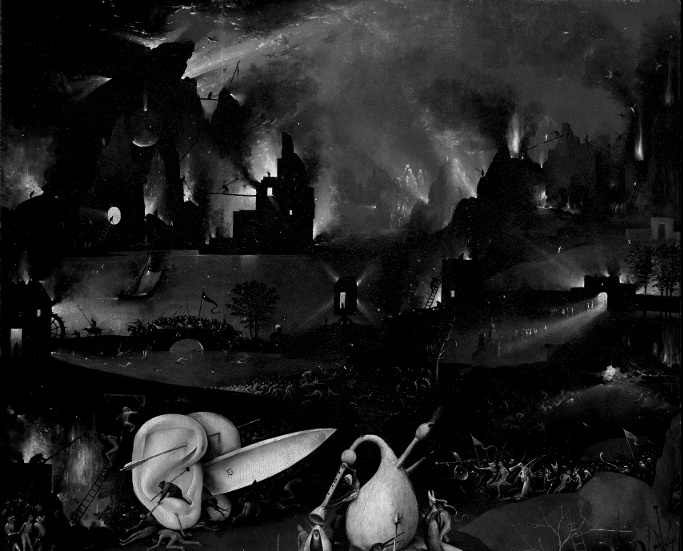
\includegraphics[width=\textwidth]{images/C1.png}
    \caption{L'enfer : des crépitements et sons discordants peuplent cette scène.}
    \label{fig.c1}
\end{subfigure}~\\
\begin{subfigure}[t]{\textwidth}
    \centering
    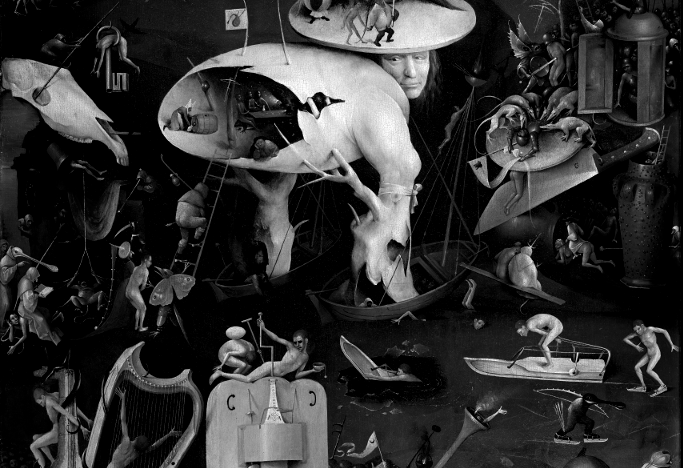
\includegraphics[width=\textwidth]{images/C2.png}
    \caption{Les personnages de cette scène vont peu à peu s'énerver au fil des interactions qu'a le public.}
    \label{fig.c2}
\end{subfigure}~\\
\begin{subfigure}[t]{\textwidth}
    \centering
    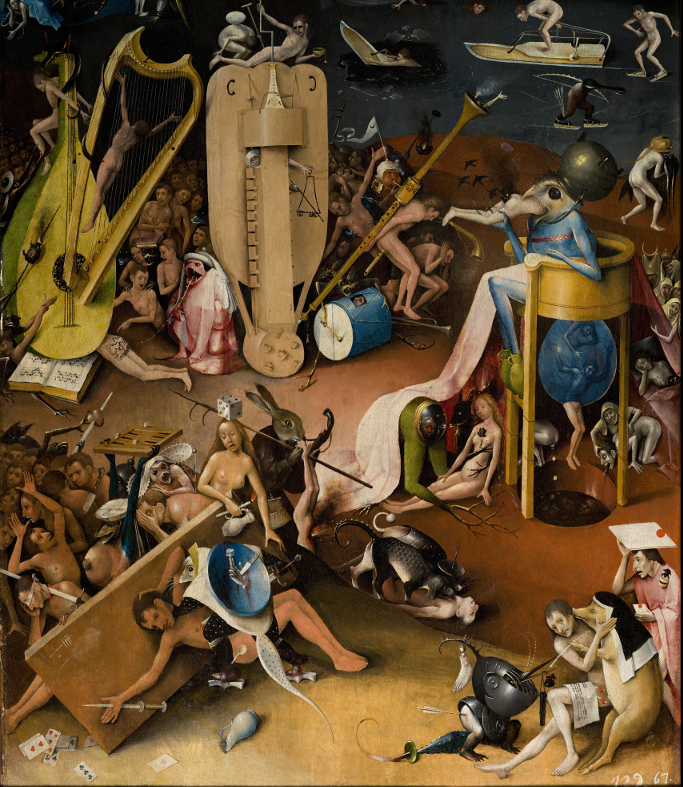
\includegraphics[width=\textwidth]{images/C3.png}
    \caption{Cette scène permet une interaction musicale avec les instruments, par le biais d'un moteur de synthèse granulaire.}
    \label{fig.C3}
\end{subfigure}
\end{subfigure}
        \caption{Panneau droit}
    \end{figure}
    \begin{figure*}
        \centering
        \begin{subfigure}[t]{\textwidth}
    \centering
    \begin{subfigure}[t]{\textwidth}
\centering
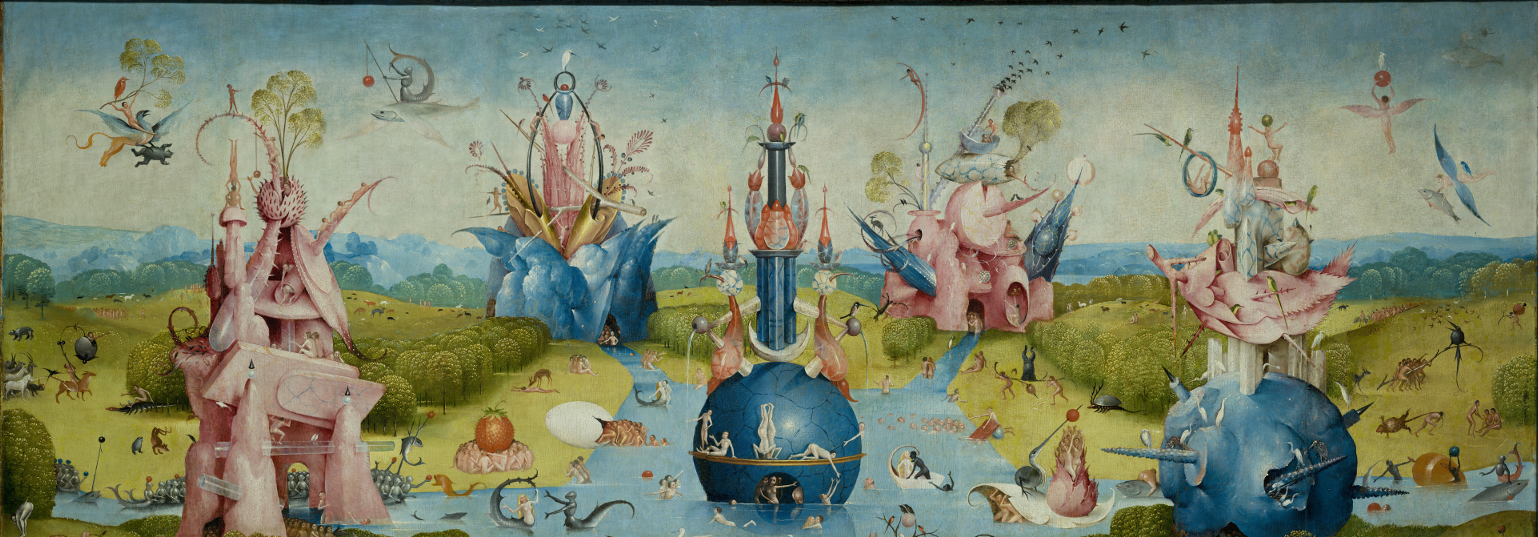
\includegraphics[width=\textwidth]{images/B1.png}
\label{fig.b1}
\caption{Les cinq structures font office d'instrument de musique spatialisé : chacun produira un son à une hauteur différente. Lorsque le premier est activé, des effets commencent à s'appliquer sur le son.}
    \end{subfigure}~\\   
    \begin{subfigure}[t]{\textwidth}
\centering
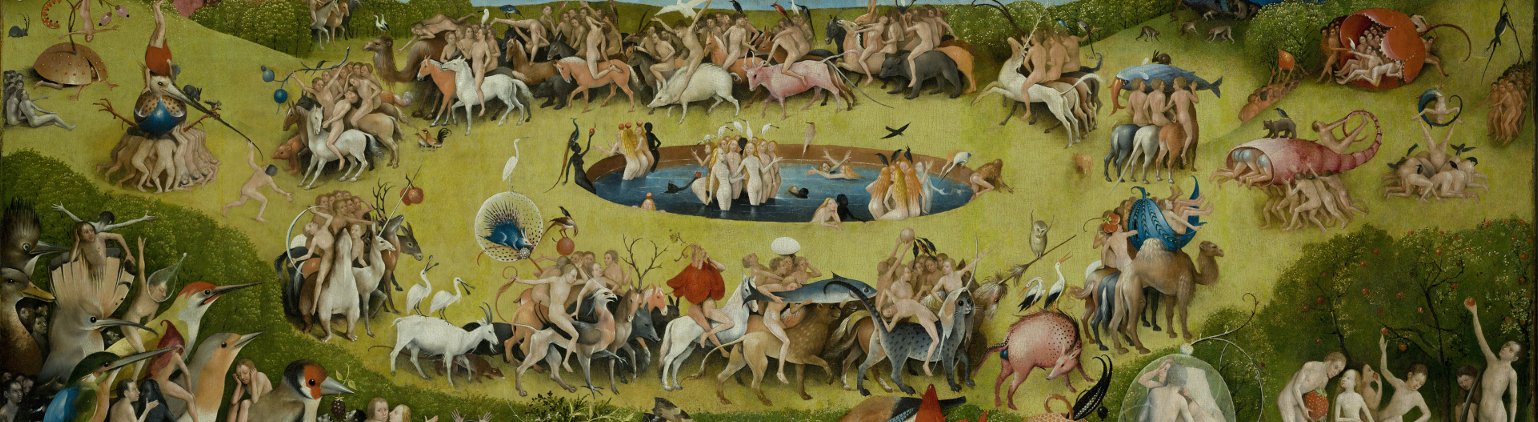
\includegraphics[width=\textwidth]{images/B2.png}
\caption{Il est possible d'explorer cette scène en naviguant dans son espace; le mouvement invite à l'utilisation de trajectoires spatialisées qui sont implémentées à l'aide d'automations tridimensionnelles dans i-score.}
\label{fig.b2}
    \end{subfigure}~\\  
    \begin{subfigure}[t]{\textwidth}
\centering
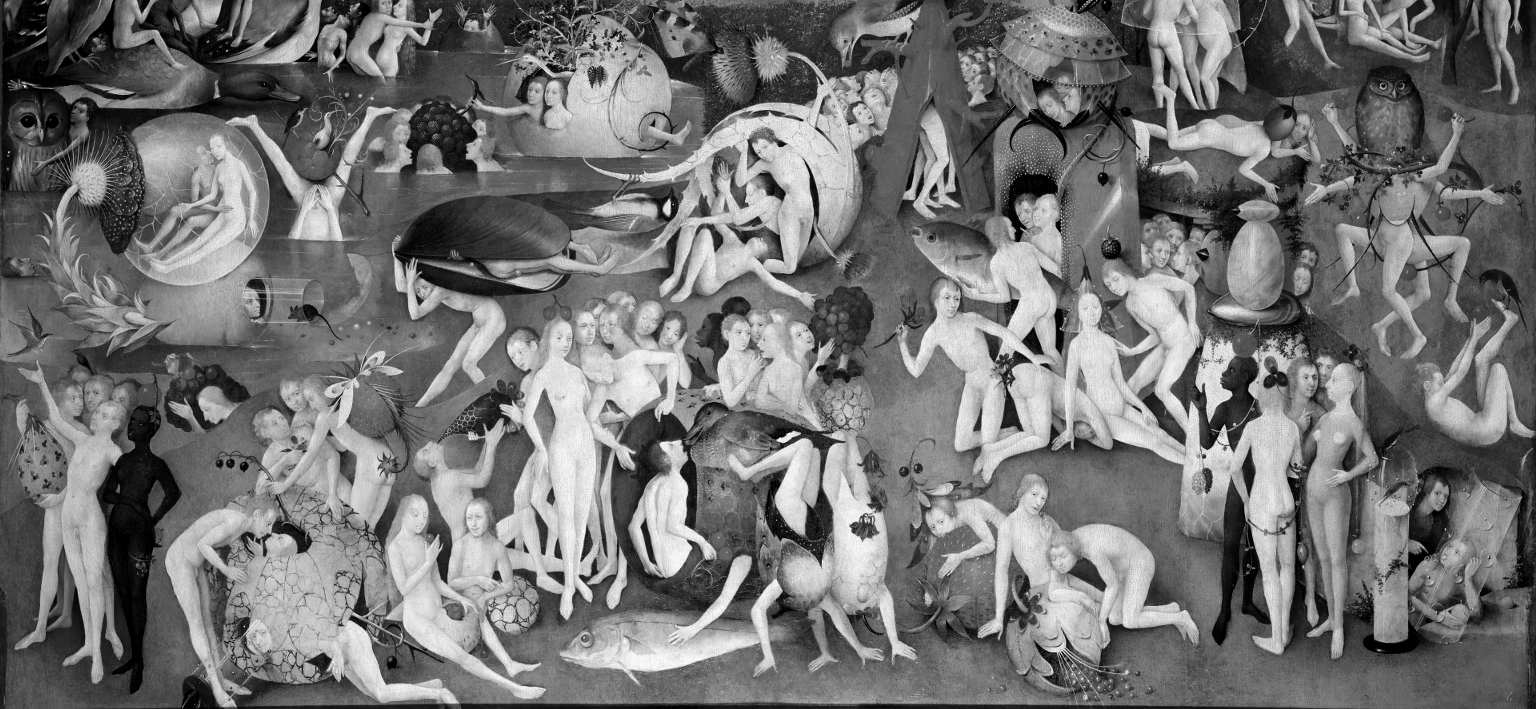
\includegraphics[width=\textwidth]{images/B3.png}
\caption{Dans cette partie, des acteurs se déplacent en permanence; interagir avec certains d'entre eux aura des effets sur une trame globale pour cette scène, ainsi que pour l'ensemble du panneau.}
\label{fig.b3}
    \end{subfigure}  
    \label{fig.b}
\end{subfigure}
        \caption{Panneau central}
    \end{figure*}
}
    
\end{document}
